\subsection{Personalizacion}
So far we have seen different parameters to consider the relevant data at a general level, in this section, we
We will focus on a personal level.
Each user is unique as well as their personal situation, so we will have to find a way to get the data
adapt to users. Offer you information not only relevant at a general level but at a particular level.
Posing that we need to be told the data in my case, by the place where I live, by
my health, family situation, something that characterizes us can help us.

In many cases, we will not be able to fully customize it, but we can look for common points in subgroups of
users, from this point you have to study the different cases that can be given and make a selection of those that are
more common.

The key question to be able to personalize the information according to the users is to ask ourselves how they could be
relate the data at a specific time, in a specific place to meet specific needs of the
user as an individual.

\subsubsection{How to solve it} 

Study in what way the data will help the user or the subgroups and from this point, make it more specific, in this way
  we will go from obtaining relevant data in a general way to be relevant in a personal way. You have to think about the
  user, not the users and find a way to find the results that are specifically adapted to him in a
  moment and place determined.

\subsubsection{How we solve it. Aire Guru} 
 We are all interested in the pollution that surrounds us, since it is important for our health, for this reason, the tool
 Aire Guru has specialized in this area. For those people who are especially sensitive to the pollution of the
 Air, Air Guru shows the air pollution with respect to the six most common medical conditions that
 they are affected by some contaminant.
 

\begin{figure}[ht]
    \centering
   \subfigure[EPOC]
    {\includegraphics[width=3.5cm  ]{filter_epoc}}
    \hfill
    \subfigure [Asthma]
       { 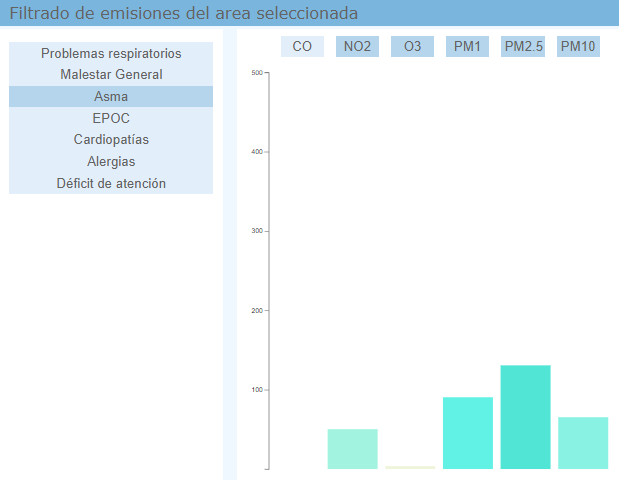
\includegraphics[width=3.5cm]{filter_asthma}}
    \hfill
     \subfigure[Allergies]
     {   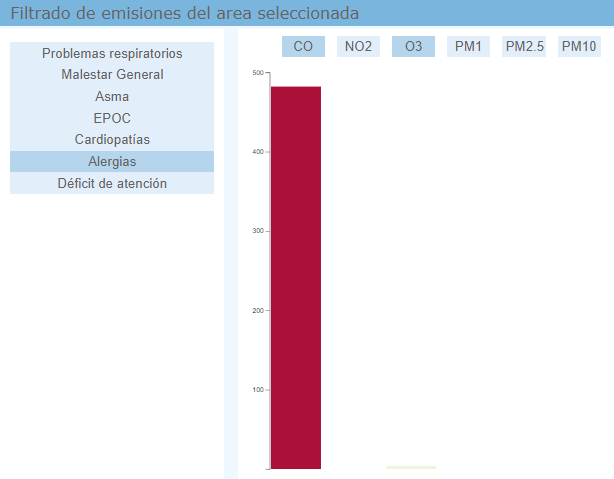
\includegraphics[width=3.5cm]{filter_allergies}}
  
  \caption{Medical Condition Filter}
    \end{figure}
    As we see, in each of the cases, for each medical condition, it shows a subset of pollutants,
      those that most influence each medical condition.
    
    The answer to the key question, how can I relate the data to a specific time and place, does not lead to
    implementation of a personal history of exposure to pollution. That is, to know at all times what pollution
    I am submitted and in what place it happened.
    For this, it is very essential to read the user's position, with the confrontation of the location of the
    user and the coordinates provided by the original dataset, we can find the level of exposure to contamientamentes,
    If the user gives us his permission to store this data, we can show him his personal history.
    \begin{figure}[ht]
      \centering 
      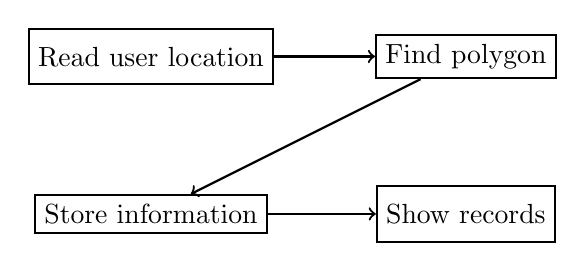
\begin{tikzpicture}[thick]
          \node[draw,rectangle,minimum size=20] (a) {Read user location};
           \node[draw,rectangle,minimum size=6,right of= a, node distance=4cm] (b) {Find polygon};
           \node[draw,rectangle,minimum size=5,below of= a, node distance=2cm] (c) {Store information};
           \node[draw,rectangle,minimum size=20,right of=c, node distance=4cm] (d) {Show records};
           \draw[->] (a) to (b);
          \draw[->,] (b) to (c);
          \draw[->] (c) to (d);
     
        \end{tikzpicture}
        \caption{Collecting user location}
      \end{figure}

      This functionality is the most relevant of the Air Guru tool, since for other platforms, this functionality is not
      possible if user-level measurement devices are not used, that is, the user has to always carry
      a measurement station that monitors the different pollutants. \\
      \begin{figure}[ht]
         \centering
         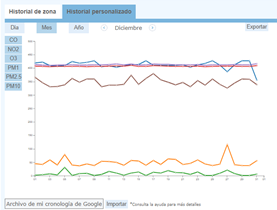
\includegraphics[width=8cm]{importedDataDecember}
         \caption{Personal Records. December}
     \end{figure}
     As we are aware that user may have started to use the application and have no available data,
     you are offered the possibility of importing the Google location history, in this way, you will be able to visualize
     Exposure to pollution since the beginning of 2018 even if you have not been using the tool.
     
     We will have to take into account that in order to read the user's position and store their data, we must
     have their explicit permission and implement mechanisms that provide us with the necessary security to not put
     risk the data of our users. The measures taken will be explained later.
     
     


\elsparagraph{Evaluation}  
\begin{itemize}
  \done The user has specialized functionalities
     \done Unique functionality, the user is able to see the pollution to which he has been exposed since 2018 including
     without having been using the tool
     \crossed The filtering function of the medical condition is not self-selected, this is because the functionality
     It is available to all users. It could be implemented so that the map would show the AQI with respect to the
     contaminants that the user has preselected, but this can de-virtualize the information if it is not
     clearly indicates to the user that the map does not take into account all relevant contaminants.
\end{itemize}
 \newpage